\section{Java application}
\label{chapter2}

Above solutions are implemented in Java using Netbeans and SceneBuilder. This application provides GUI which allows user to alter $x_0$, $y_0$, $X$ and grid size $n$ in constraint, i.e. $x_0, X \neq 0$, $\frac{x_0+y_0}{x_0} > 0$ (to ensure that $f(x,y)$ is defined) and $X > x_0$, $n\in N$, $n > 0$. Since $f(x,y)$ is not defined at $x=0$, for the ease of implementation, I applied one more constraint to user input: $x_0$ and $X$ must have the same sign (both positive or both negative).

\subsection{User guide}

\textbf{Highlight features}
\begin{itemize}  
\item Allow changing initial values $x_0$, $y_0$, $X$ and grid size $N$.
\item Allow choosing methods: exact solution, Euler method, improved Euler method and Runge-Kutta method.
\item Provide visualization for solutions, local errors and global errors for chosen methods.
\end{itemize}

\begin{figure}[H]
	\centering
	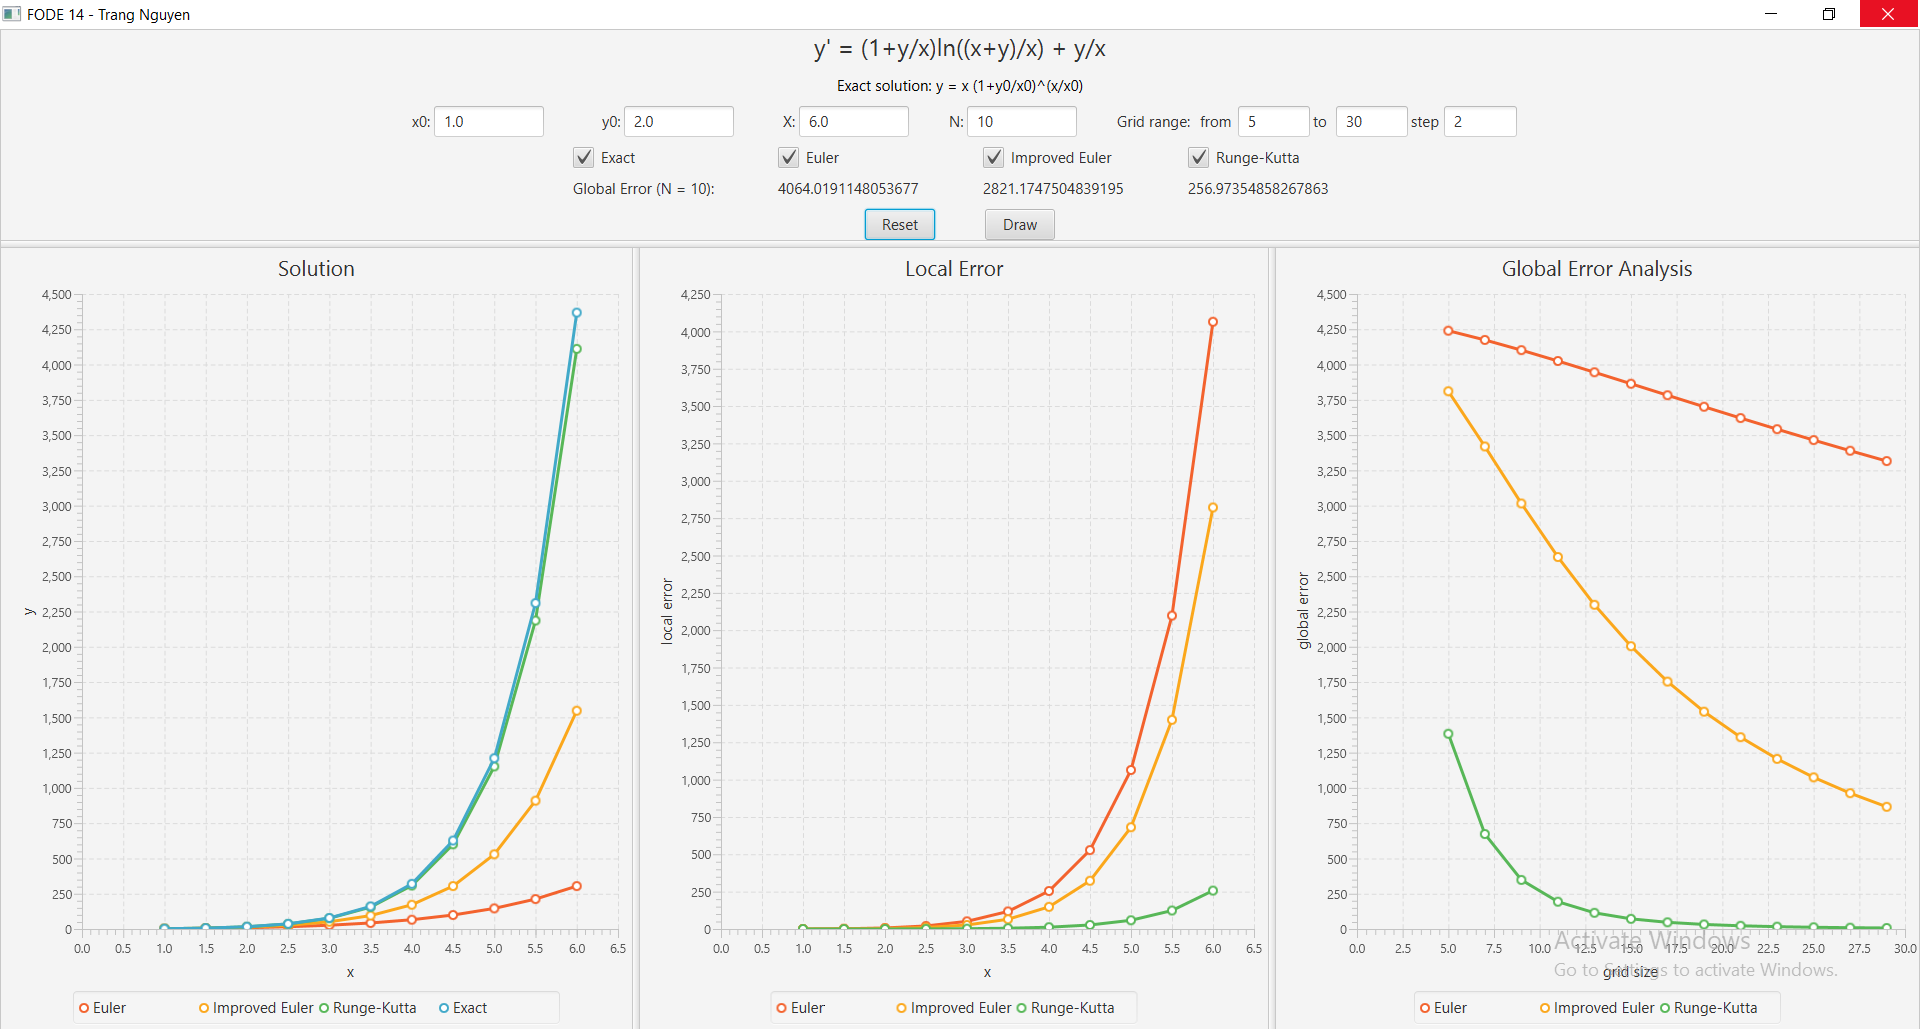
\includegraphics[width=\linewidth]{image/full.png}
	\caption{Application screenshot with default values}
	\label{fig:applicationscreenshot}
\end{figure}

\textbf{How to use}
\begin{enumerate}  
\item Enter valid initial values $x_0$, $y_0$, and $X$, grid size $N$ and grid range. Default values: $x_0=1.0$, $y_0=2.0$, $X=6.0$, $N=10$ and grid range from 5 to 30 with step of 2. Any invalid input will be informed.
\begin{figure}[H]
	\centering
	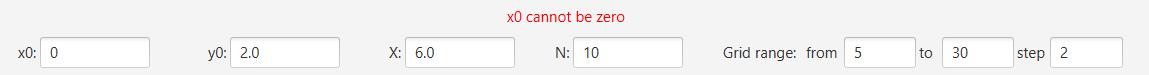
\includegraphics[width=0.8\linewidth]{image/error.png}
	\caption{Enter values}
	\label{fig:entervalues}
\end{figure}
\item Choose methods to process. Both Exact, Euler, Improved Euler and Runge-Kutta are chosen by default.
\begin{figure}[H]
	\centering
	
\includegraphics[width=0.8\linewidth]{image/method.png}
	\caption{Choose methods}
	\label{fig:choosemethods}
\end{figure}
\item Click 
\includegraphics[height=2\fontcharht\font`\B]{image/draw.png} button to start analyzing. \\Global errors with specified $N$ will be presented right below chosen methods.
\begin{figure}[H]
	\centering
	
\includegraphics[width=0.8\linewidth]{image/global.png}
	\caption{Global Errors at $N$}
	\label{fig:globalerror}
\end{figure}
Also, plots of solutions, local errors, global errors in grid range will be updated in drawing space.
\begin{figure}[H]
	\centering
	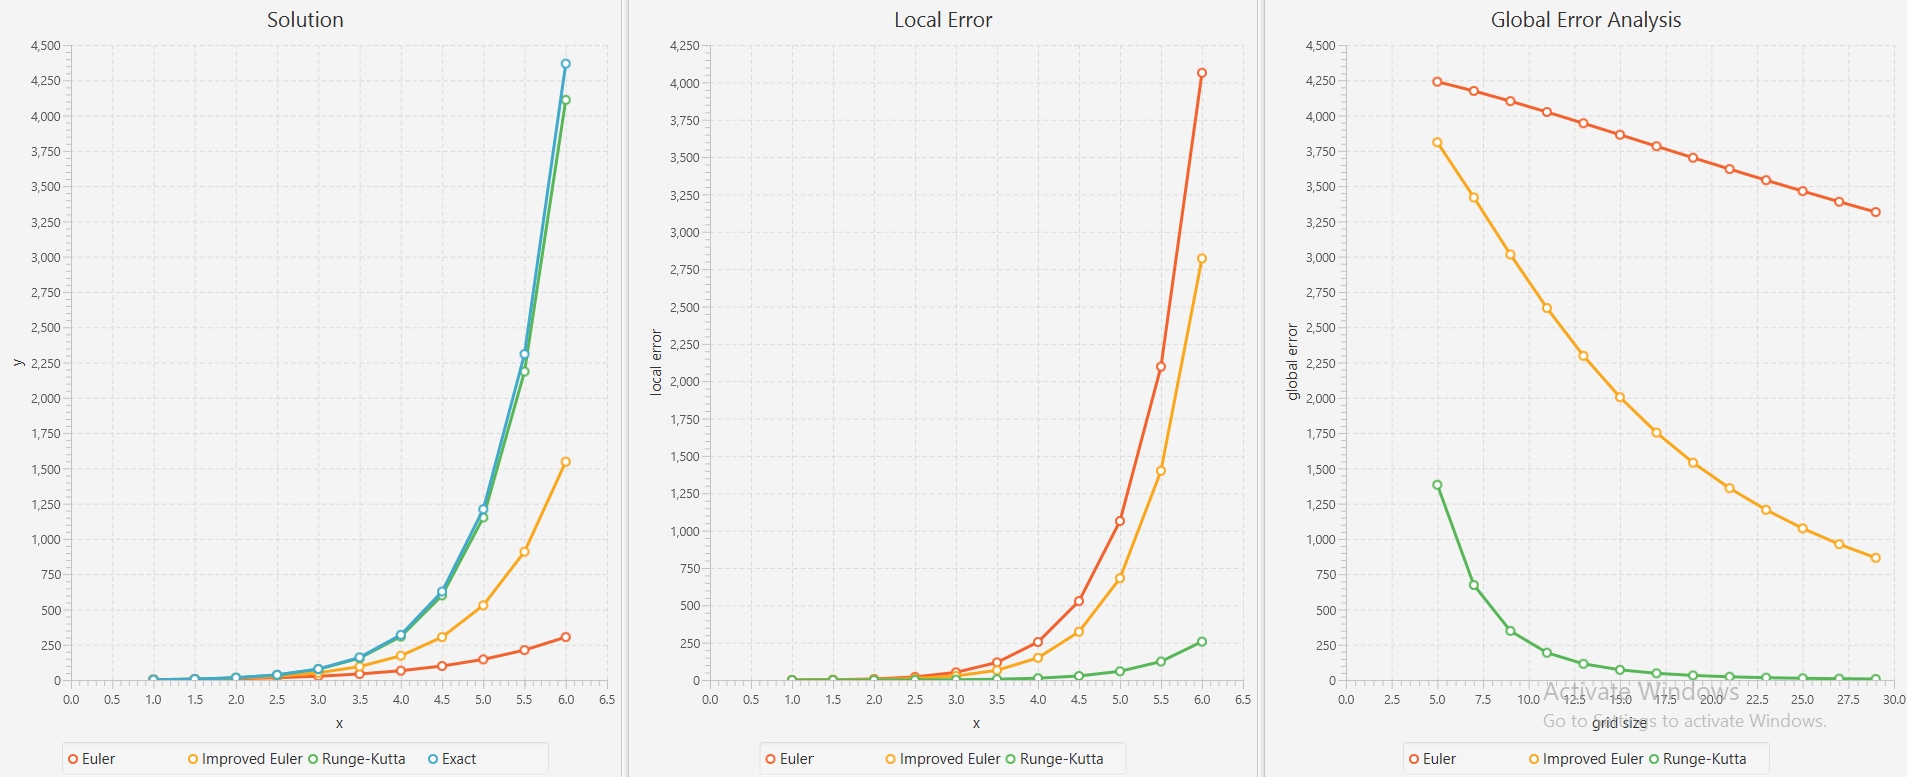
\includegraphics[width=\linewidth]{image/plot.png}
	\caption{Plots of solutions, local errors at $N$; and global errors in grid range}
	\label{fig:plot}
\end{figure}

\end{enumerate}
Click 
\includegraphics[height=2\fontcharht\font`\B]{image/reset.png} button to reset all elements to default values.

\subsection{Implementation}

The application is written in Java using Netbeans and SceneBuilder. Since for each initial value $x_0$, and $y_0$; and $X$, exact solution and it's approximation should be provided, I decided to used only one class named Fode14 for our ODE. In GUI, there is only two event handlers (for clicking "Draw" and "Reset" buttons) which are in FXMLDocumentController class.

\begin{figure}[H]
	\centering
	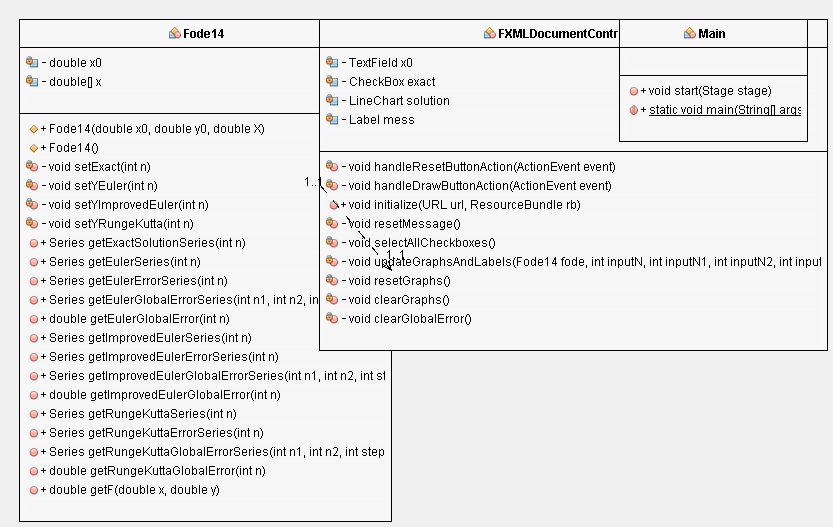
\includegraphics[width=\linewidth]{image/uml.png}
	\caption{UML Diagram}
	\label{fig:uml}
\end{figure}

Below is implementation of Runge-Kutta method (as functions in Fode14). It's structure is applicable for others.
\begin{lstlisting}
    private void setYRungeKutta(int n) throws Exception {
        setExact(n);
        
        if (yRungeKutta == null || yRungeKutta.length != n+1) {
            yRungeKutta = new double[n+1];
            yRungeKutta[0] = y0;

            double k1, k2, k3, k4;
            double h = (X-x0)/n;
            for (int i = 0; i < n; ++i) {
                k1 = getF(x[i], yRungeKutta[i]);
                k2 = getF(x[i] + h/2.0, yRungeKutta[i] + h*k1/2.0);
                k3 = getF(x[i] + h/2.0, yRungeKutta[i] + h*k2/2.0);
                k4 = getF(x[i] + h, yRungeKutta[i] + h*k3);
                yRungeKutta[i+1] = yRungeKutta[i] + h*(k1+2*k2+2*k3+k4)/6.0;
            }
        }
    }
    
    public Series getRungeKuttaSeries(int n) throws Exception {
        Series rungeKutta = new Series();
        rungeKutta.setName("Runge-Kutta");
        
        setYRungeKutta(n);
        for (int i = 0; i <= n; ++i) {
            rungeKutta.getData().add(new XYChart.Data(x[i], yRungeKutta[i]));
        }
        return rungeKutta;
    }
    
    public Series getRungeKuttaErrorSeries(int n) throws Exception {
        Series rungeKutta = new Series();
        rungeKutta.setName("Runge-Kutta");
        
        setYRungeKutta(n);
        for (int i = 0; i <= n; ++i) {
            rungeKutta.getData().add(new XYChart.Data(x[i], yExact[i] - yRungeKutta[i]));
        }
        return rungeKutta;
    }
    
    public Series getRungeKuttaGlobalErrorSeries(int n1, int n2, int step) throws Exception {
        if (n1 <= 0 || n2 <= 0 || n1 >= n2 || step <= 0) {
            throw new Exception("Invalid Grid range input");
        }
        Series rungeKutta = new Series();
        rungeKutta.setName("Runge-Kutta");
        
        for (int i = n1; i <= n2; i += step) {
            rungeKutta.getData().add(new XYChart.Data(i, getRungeKuttaGlobalError(i)));
        }
        
        return rungeKutta;
    }
    
    public double getRungeKuttaGlobalError(int n) throws Exception {
        setYRungeKutta(n);
        return yExact[n] - yRungeKutta[n];
    }
\end{lstlisting}